The FCC-ee interaction region (IR) is designed to reach the highest luminosities 
at all centre-of-mass energies, from the \PZ pole to the $\ttbar$ threshold. 
This design is based on the crab-waist collision scheme, 
with nano-beams at the interaction point (IP), 
large horizontal crossing angle, and crab-waist sextupoles~\cite{Raimondi:2007vi}. 
The Machine Detector Interface (MDI) of FCC-ee has a 
compact and complex design~\cite{FCC-PED-FSR-Vol2,Boscolo:2024bxm} 
that fulfils constraints imposed by 
the machine~\cite{FCC-PED-FSR-Vol2} and detector requirements (Chapter~\ref{sec:requirements}). 

The main beam parameters are recalled in Table~\ref{tab:IR_parameters},
for the four main operational centre-of-mass energies.
In FCC-ee, the two beams circulate in different vacuum chambers, which merge at 1.3\,m from the IP. 
The distance between the face of the  superconducting final focus quadrupole (FFQ) 
and the IP (${\ell^{*}}$) is 2.2\,m, 
well inside the detector volume (Section~\ref{sec:concepts}). 
In addition to the optics constraints on the IR layout, 
physics considerations strongly advocate for hermetic detectors 
and for constraining
the accelerator components within a cone of 100\,mrad from the IP, 
along the $z$ axis\footnote{The coordinate system of the detector 
has the origin centred at the nominal collision point. 
The $z$ axis is defined as the bisector of the axes of the incoming and outgoing beams, 
ideally in the direction of the axis of the experiment solenoid. 
The $x$ axis is in the plane subtended by the two beams and pointing away from the centre of FCC. 
In this way, the positron beam is travelling towards positive values of $z$ (mainly) and $x$ (subordinately). 
Perpendicular to the $(x,z)$-plane, the $y$ axis points upwards. 
The polar angle, $\theta$, is then measured with respect to the $z$ axis 
and the azimuthal angle, $\phi$, with respect to the $x$ axis in the $(x,y)$ plane. 
The radial coordinate, $r=\sqrt{x^2+y^2}$, is the distance from the $z$ axis.}.
These requirements demand a compact MDI design with tight space constraints.

\begin{table}[ht]
\centering
\caption{Key collider parameters for the FCC-ee IRs with 4 IPs.
The bunch length, $\sigma_{z}$, is different for non-colliding bunches (determined by `synchrotron radiation', SR) 
and colliding bunches (determined by `beamstrahlung', BS); 
$\sigma_{x}^{*}$ and $\sigma_{y}^{*}$ denote the bunch sizes at the IP in the (horizontal and vertical, respectively) 
transverse directions, while $\sigma_{\delta}$ is the relative beam energy spread.}
\label{tab:IR_parameters}
\setlength{\tabcolsep}{2.5pt}
\renewcommand{\arraystretch}{0.8}
\begin{tabular}{l c c c c}
\toprule
     &  \PZ   & $\PWp\PWm$ & $\PZ\PH$ & $\ttbar$ \\ \midrule
Beam energy (GeV)              & 45.6  & 80 & 120 & 182.5  \\
Luminosity / IP ($10^{34}$\,cm$^{-2}$s$^{-1}$) & 145 & 20 & 7.5 & 1.41 \\
Beam current (mA)              & 1\,294  &  135  & 26.8  & 5.1  \\
Bunch number / beam            & 11\,200  &  1\,852 & 300   & 64      \\
Bunch spacing (ns)             & 27 & 163 & 1\,008 & 4\,725 \\
$\sigma_{x}^{*}$ ($\mu$m)      & 9.5  & 21.8 & 12.6 & 36.9  \\
$\sigma_{y}^{*}$ (nm)          & 40.1   &  44.7 & 31.6 &  43.6  \\
$\sigma_{z}$ (mm) SR / BS      & 4.7 / 14.6 & 3.46 / 5.28 & 3.26 / 5.59 & 1.91 / 2.33 \\
$\sigma_{\delta}$ (\%) SR / BS & ~0.039 / 0.121~ & ~0.069 / 0.105~ &  ~0.102 / 0.176~ &  ~0.151 / 0.184~ \\
\bottomrule
\end{tabular}
\end{table}

The crab-waist scheme requires a large horizontal crossing angle of 30\,mrad. 
The incoming beams point straight to the IP, 
while the outgoing beam trajectories are strongly bent from the IP, 
so that the beams can successfully merge back close to the opposite ring~\cite{Oide:2016mkm}. 
This scheme ensures that most of the synchrotron radiation (SR) generated at the IR magnetic elements 
does not strike the IR central beam pipe.
The intense radiation emitted during the collision in the electromagnetic field of the opposite beam, 
known as beamstrahlung (BS), is mostly collinear with the outgoing beams, similarly to the SR~\cite{Boscolo:2023grv}. 
Both the BS and SR photons are stopped at about 500\,m downstream of the IP, 
in dedicated dumps~\cite{frasca:ipac2024-tupc66}.
%
To minimise the level of SR photons that reach the detectors, 
the closest bending magnet is located at more than 100\,m from the IP 
and those located up to 500\,m have a SR critical energy below 100\,keV.

To counteract the beam rotation and deflection 
that would be caused by the simultaneous effects of the detector magnetic field of 2\,T and the crossing angle, 
a compensating solenoid delivering a magnetic field of $-5$\,T is placed at 1.23\,m from the IP, 
cancelling out the longitudinal magnetic field integral along the $z$ axis 
from the last focusing quadrupole to the IP.
Consequently, the front face of the luminosity calorimeter (LumiCal), 
placed in front of the compensating solenoid, is only 1\,m from the IP. 
The LumiCal is centred around the outgoing beam direction 
and measures the integrated luminosity from the rate of low-angle Bhabha events, $\epem\to\epem$.
%
The first layer of the vertex detector must be placed as close as possible to the IP 
to optimise the precision of the primary and secondary vertex position determination, 
with direct impact on the efficiency and purity of flavour tagging algorithms. 
The smallest affordable distance is set by the central beam pipe radius of 1\,cm. 
The length of the vertex detector (1.86\,m) is chosen to cover the angular region $|\cos\theta| < 0.99$. 
A lightweight mechanical structure is designed for its support.
To avoid any material in front of the LumiCal, 
all other detector elements must be placed above 110\,mrad with respect to the $z$ axis.

An overall design of the interaction region is shown in Fig.~\ref{fig:IR}.
The next sections describe the main features of the MDI. 
A more detailed discussion can be found in Ref.~\cite{boscolo_2023_p4vnt-2va28}.

\begin{figure}[ht]
\centering
\includegraphics[width=0.75\linewidth]{Physics/MachineDetectorInterface/Figs/MDI_layout1.pdf}
\caption{Layout of the interaction region. 
The support tube allows the integration of the luminosity calorimeter (LumiCal) and the vertex detector. 
The three segments of the final focus quadrupoles (QC1) are shown with the screening and compensating solenoids.}  
\label{fig:IR}
\end{figure}

\subsection{Interaction region layout}

The mechanical layout of the IR comprises an 18\,cm long central beam pipe with a 10\,mm internal radius, 
a pair of ellipto-conical beam pipes about 1064\,mm long on either side, 
a silicon vertex detector covering the radial range from 13.7 to 315\,mm, 
and the LumiCal at 1074\,mm from the IP, 190\,mm thick, covering the angular range between 50 and 134\,mrad.
All these elements are held in place by a lightweight carbon fibre and honeycomb rigid structure support tube,
which allows the overall integration before the insertion in the experiment~\cite{Boscolo:2023hwo}.
The vacuum chambers are made of AlBeMet162, an alloy of Aluminium (38\%) and Beryllium (62\%),  
chosen for its high elastic modulus and low density. 

The central beam pipe has a double layer structure, 
cooled by liquid paraffin flowing between the two layers, 
as displayed in Fig.~\ref{fig4:central}. 
A cross-sectional view of the central beam pipe and of the cooling manifolds, 
also made of AlBeMet162, is shown in Fig.~\ref{fig4:central} as well.
The double-layer structure is made of two concentric cylinders, 
each one 0.35\,mm thick and assembled with 1\,mm gap for the paraffin flow, 
thus bringing the effective diameter of the central beam pipe and its cooling layer to 23.4\,mm.
An internal 5\,$\mu$m coating layer of gold ensures a good electrical conductivity 
to minimise the beam heat load to nearly 60\,W~\cite{Novokhatski:2023wyf}
and to shield the vertex detector from residual high energy SR photons.

\begin{figure}[t!]
\centering
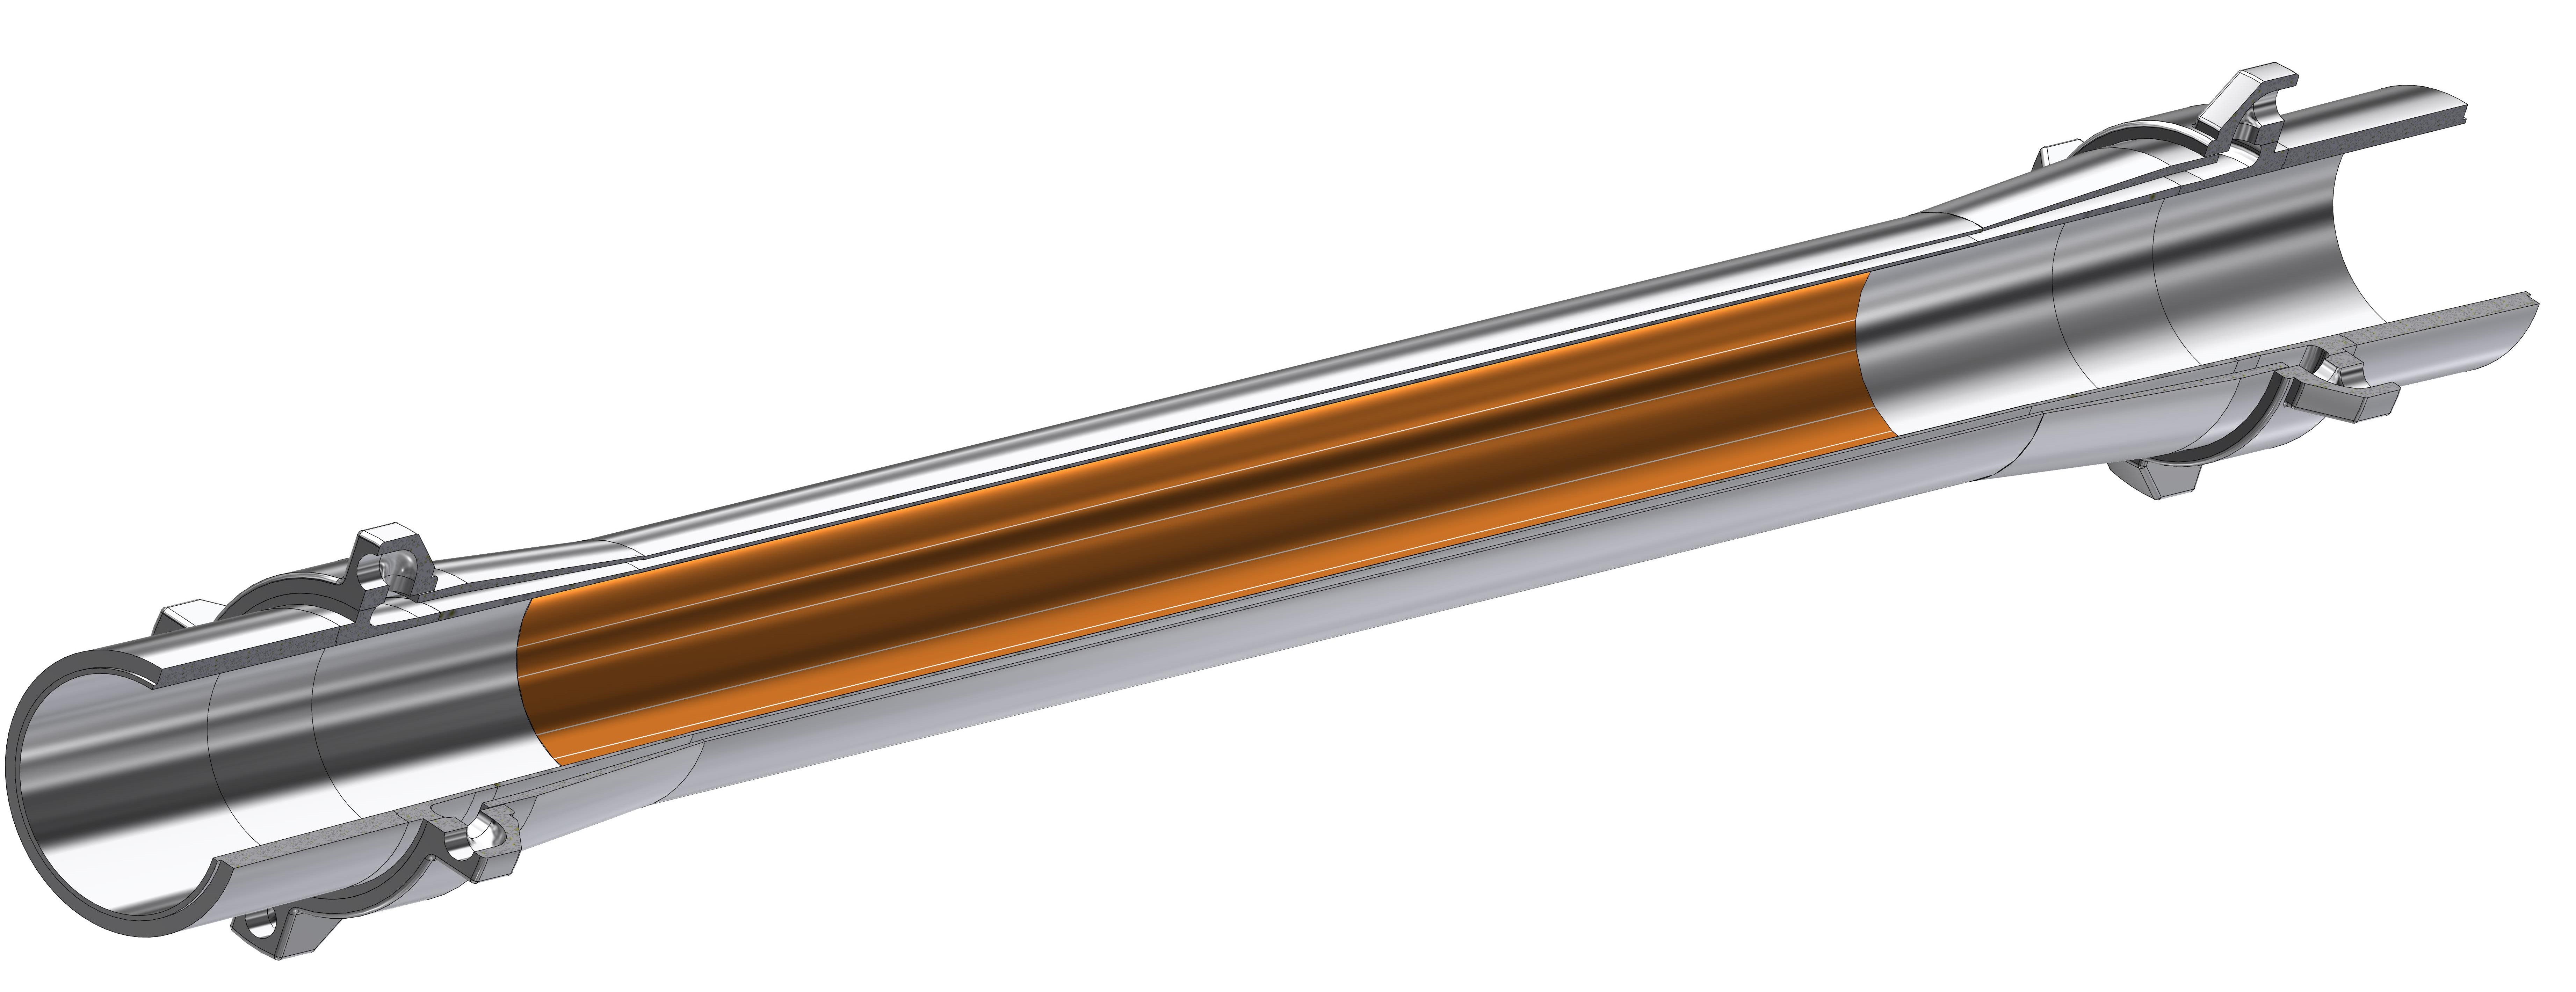
\includegraphics[width=0.45\linewidth]{Physics/MachineDetectorInterface/Figs/central_chamber.jpg}
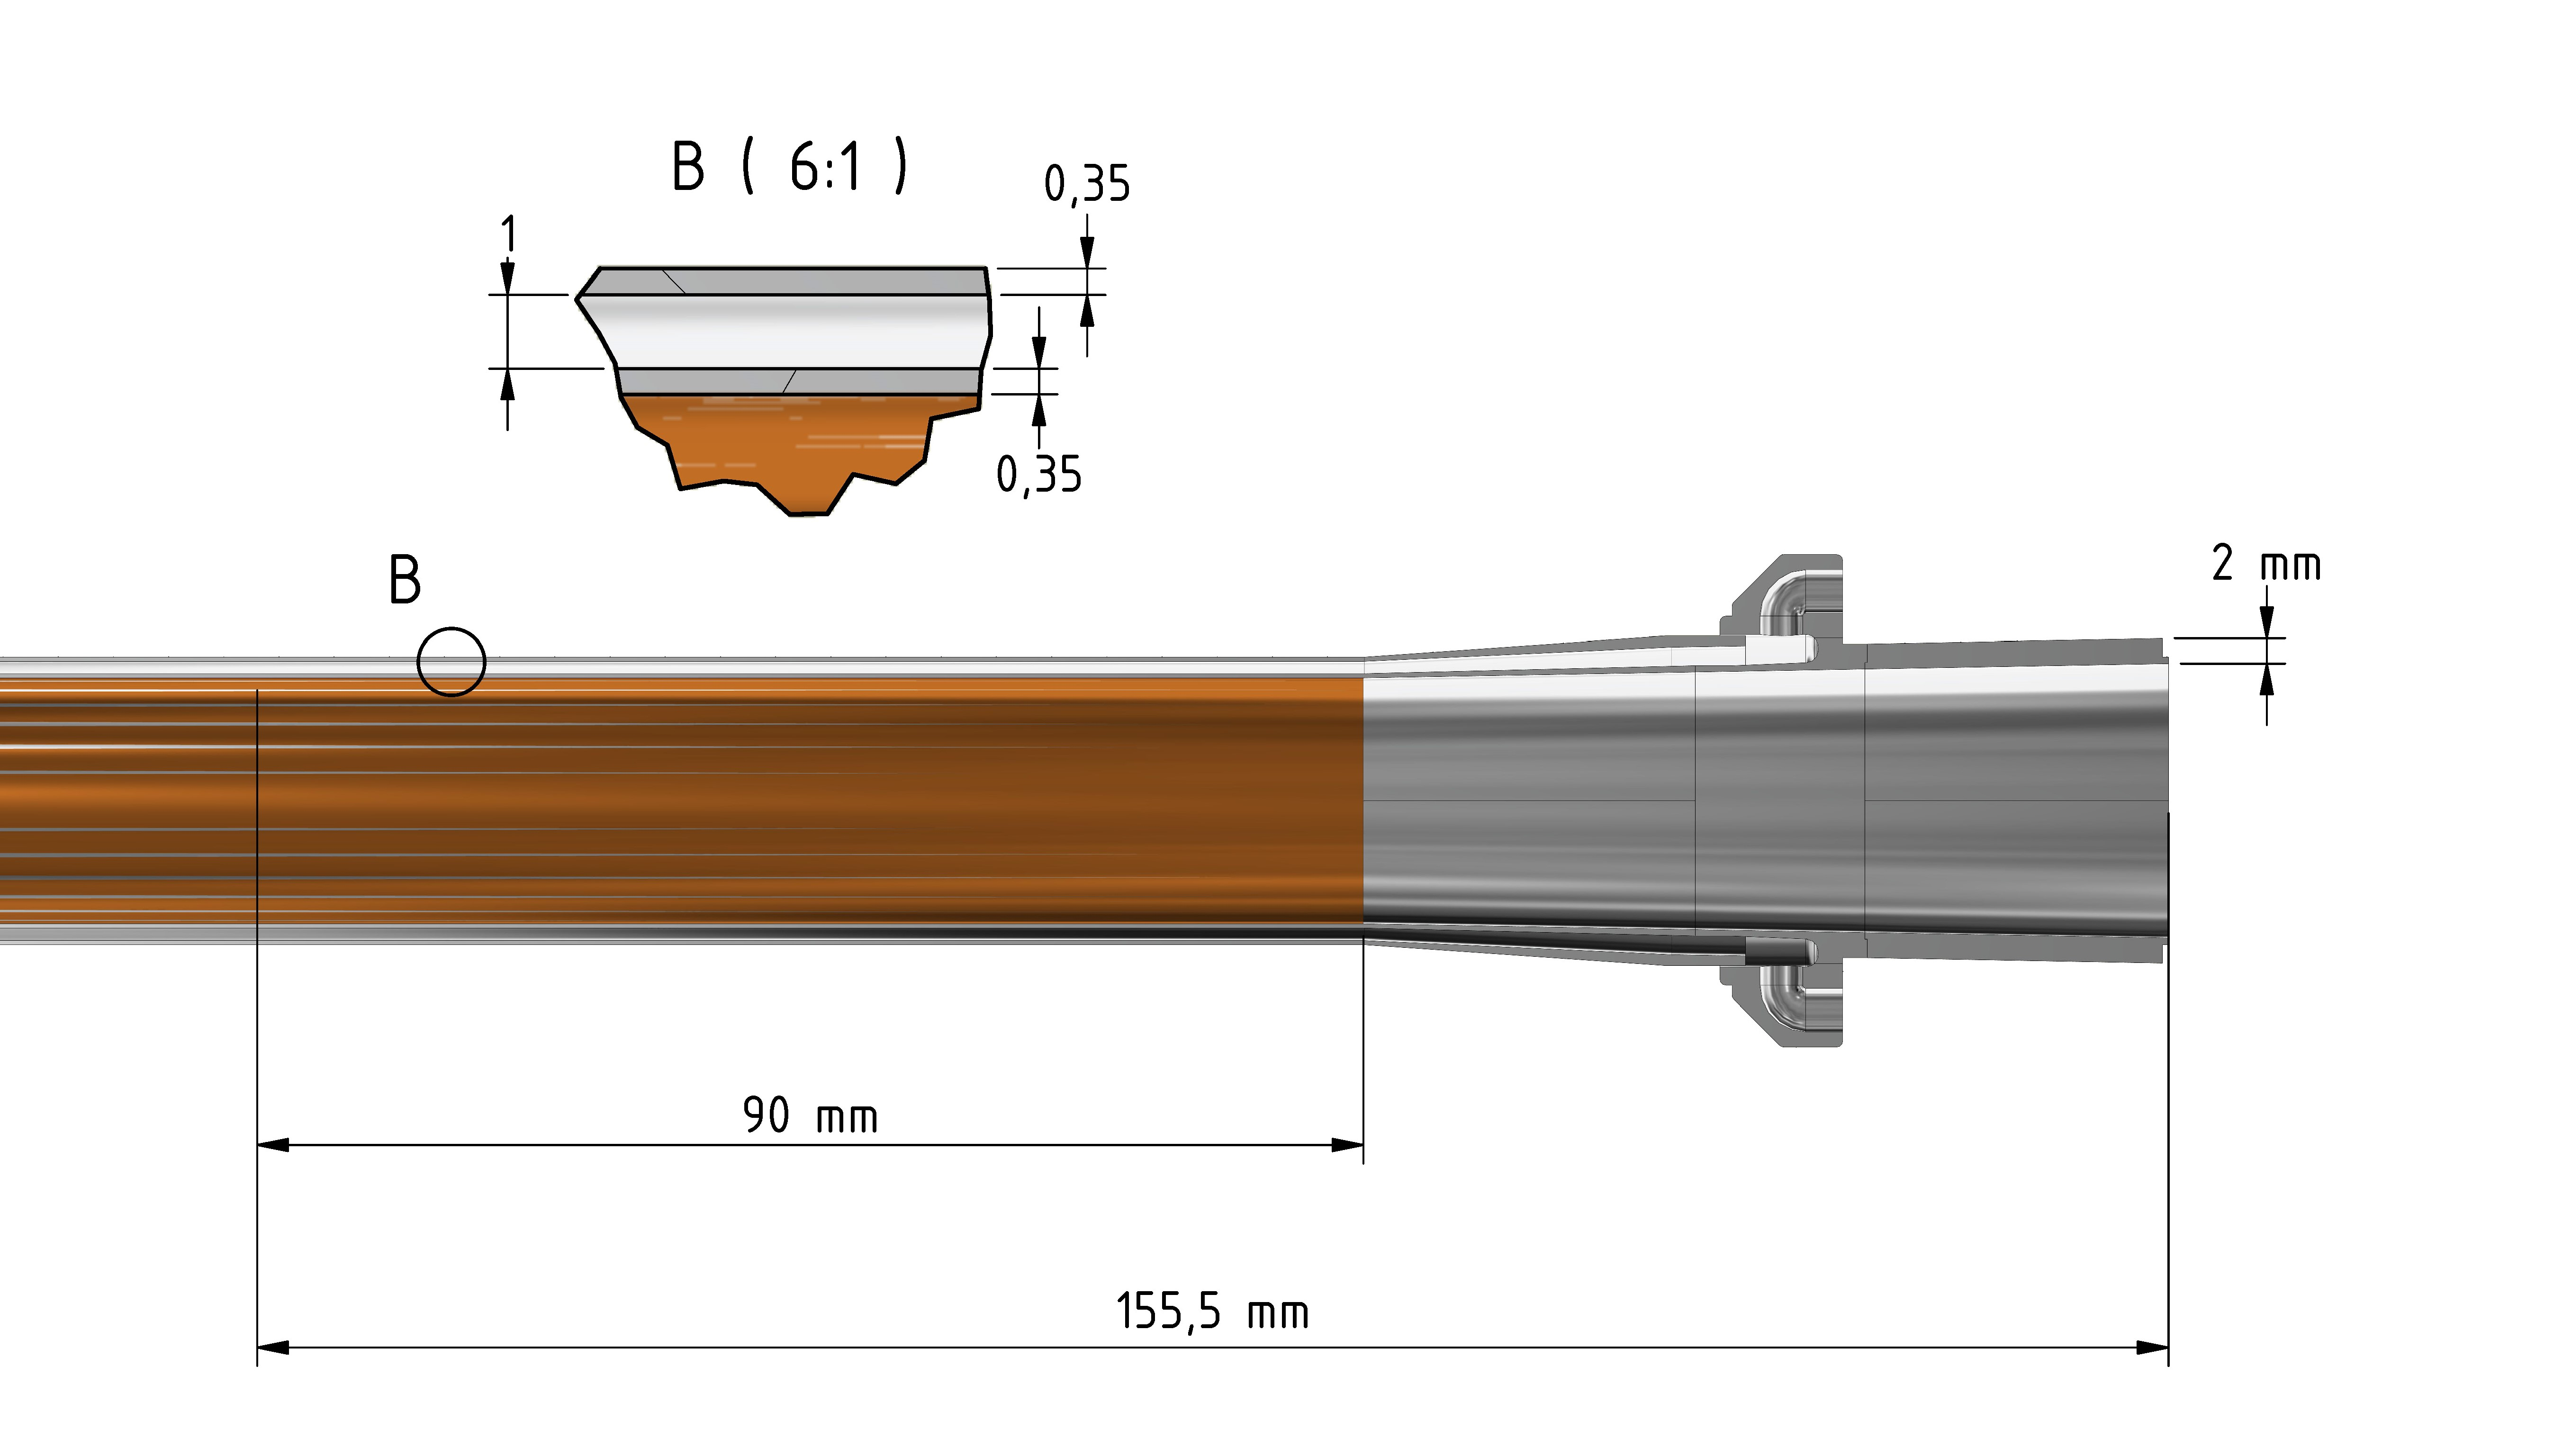
\includegraphics[width=0.39\linewidth]{Physics/MachineDetectorInterface/Figs/central_chamber_1.jpg}
\caption{Left: The central chamber in AlBeMet162 with its cooling inlets and outlets, 
and its internal gold coating layer. 
Right: Chamber cross section and zoom on the cooling channel for the paraffin flow.}  
\label{fig4:central}
\centering
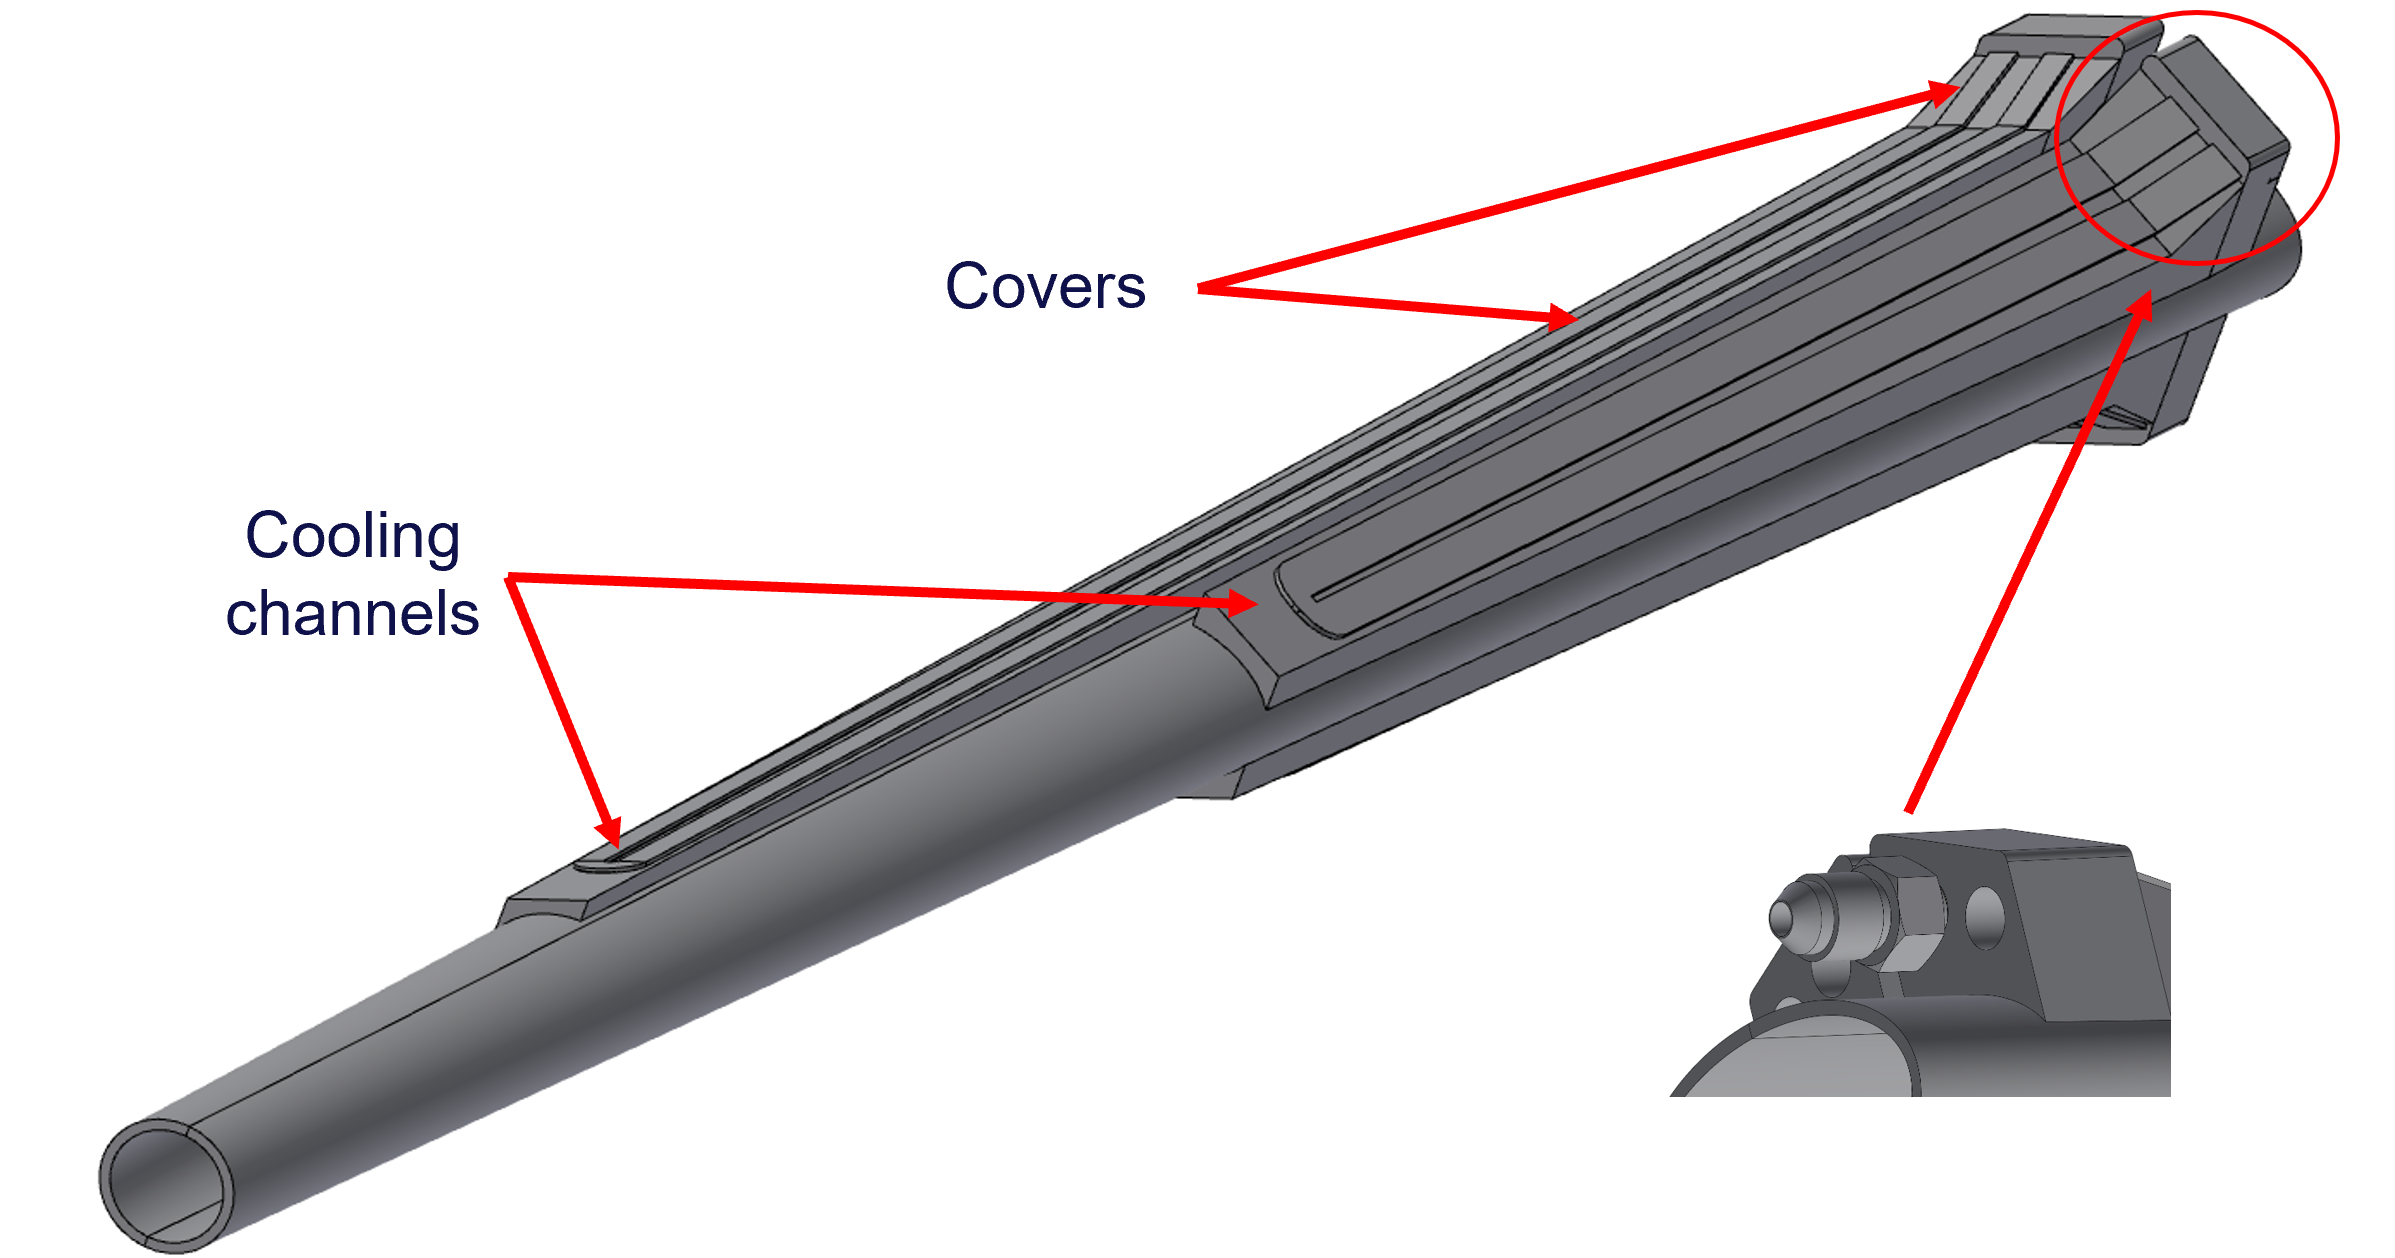
\includegraphics[width=0.6\textwidth]{Physics/MachineDetectorInterface/Figs/ellitpo_chamber.png}
\caption{Ellipto-conical vacuum chamber.}
\label{fig5:ellipto_chamber}
\centering
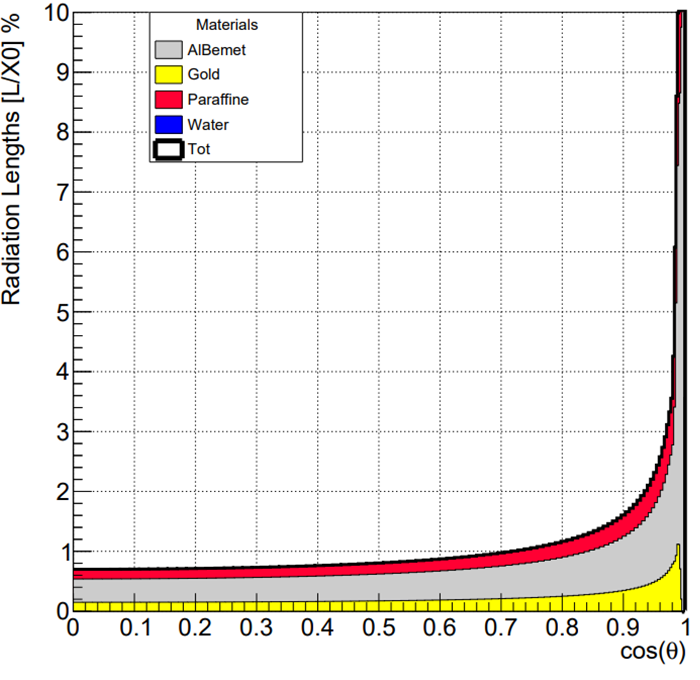
\includegraphics[width=0.45\linewidth]{Physics/MachineDetectorInterface/Figs/material_budget_AlBeMet_alltheta.png}
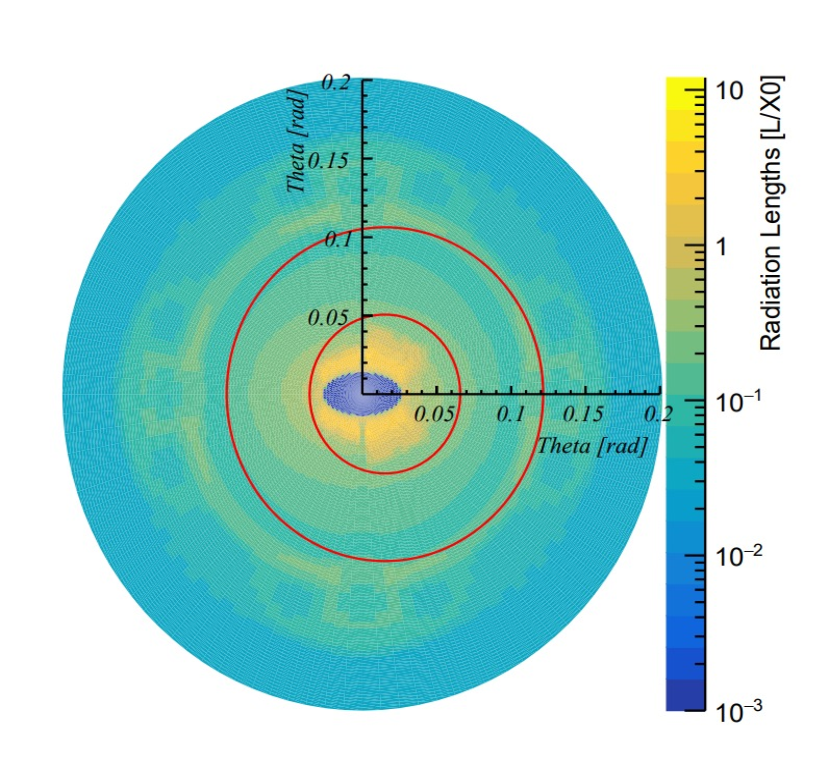
\includegraphics[width=0.5\linewidth]{Physics/MachineDetectorInterface/Figs/material_budget_albemet_manifolds_round.pdf}
\caption{Left: Material budget of the beam pipe, in per cent of a radiation length,
as a function of the $\cos\theta$ polar angular.
Right: Distribution of the material budget of the beam pipe in the transverse plane,
in the $0 < \theta < 0.2$\,rad angular range, at the entrance of the LumiCal. 
The red lines represent the LumiCal angular coverage.}
\label{fig:material_budget_Gold_5mum}
\end{figure} 

The ellipto-conical vacuum chamber, shown in Fig.~\ref{fig5:ellipto_chamber},
extends between 90 and 1154.5\,mm from the IP. 
Following a short transition from the central chamber, its thickness remains at a constant value of 2\,mm. 
Water flows in the cooling channels to extract an expected heat load of about 130\,W; 
an asymmetric design is needed to match the angular acceptance of the luminosity calorimeter.

A thermo-structural analysis has been performed to calculate the temperature distribution, 
stress, strain and displacement of the beam pipes.
The maximum temperature of the central chamber reaches 29\,$^{\circ}$C, 
cooled with paraffin entering at 18\,$^{\circ}$C , 
while it amounts to 50\,$^{\circ}$C for the conical chamber cooled with water entering at 16\,$^{\circ}$C. 
The maximum stress has been calculated considering the constraint configurations of a cantilevered support, 
resulting in a maximum displacement of 0.5\,mm 
and a maximum stress ten times lower than the AlBeMet162 yield strength (193\,MPa).
The resulting material budget distribution for the vacuum chamber 
is shown in Fig.~\ref{fig:material_budget_Gold_5mum} as a function of the polar angle.
The material encountered by a particle produced at normal incidence corresponds to 0.68\% of a radiation length ($X_0$). 

Several vertex detector designs are described in Section~\ref{sec:concepts}. 
The integration study performed here is based on the engineered version currently adopted by the IDEA concept (Section~\ref{sec:IDEA_vertex}). 
This version features two main subsystems, of active elements based on 50\,$\mu$m thick `Monolithic Active Pixel Sensors': 
an inner vertex detector, composed of three barrel layers at a radial distance between 13.7 and 35.6\,mm, 
covering an angular acceptance of about $|\cos\theta| < 0.99$; 
and an outer vertex detector, composed of two barrel layers at 13 and 31.5\,cm, and three disks on either side of the IP.

\begin{figure}[ht]
\centering
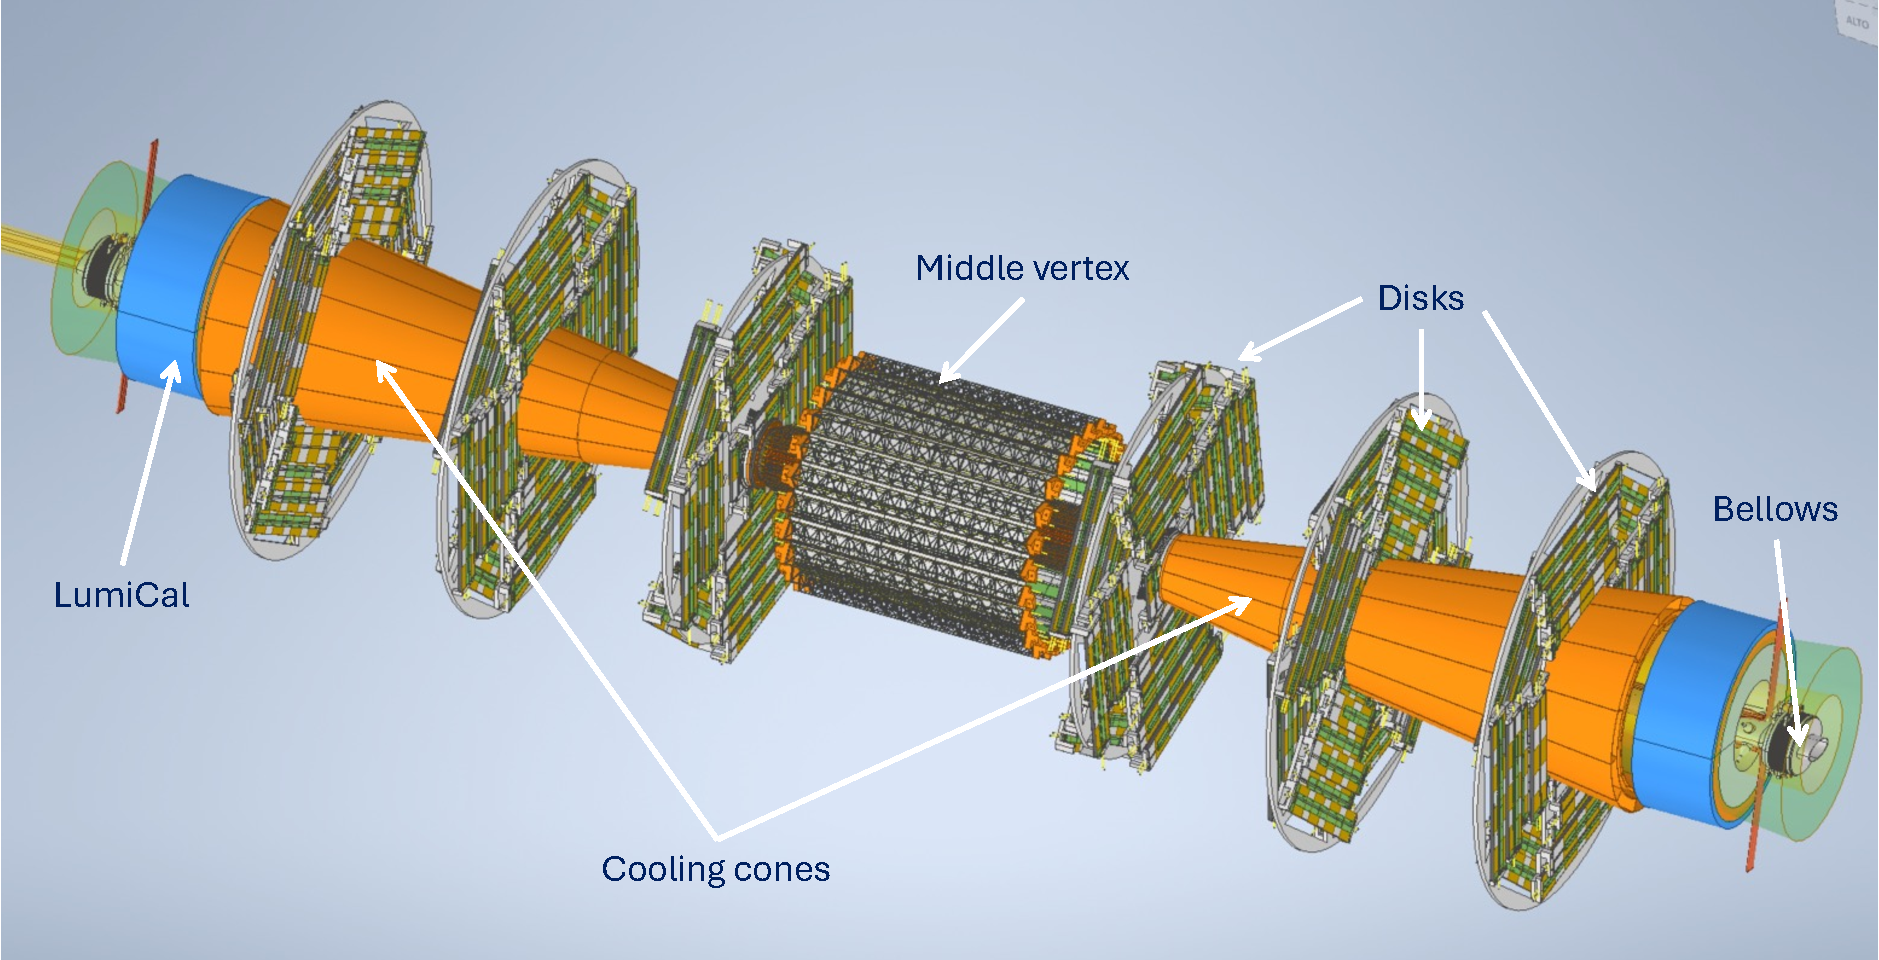
\includegraphics[width=0.8\linewidth]{Physics/MachineDetectorInterface/Figs/cones.pdf}
\caption{Layout of the vertex detector cooling cones assembly, together with the main elements to be integrated around it.}
\label{fig:cooling_cones}
\end{figure}

The inner vertex detector is cooled by flowing gas (air or helium) through a system of carbon fibre cones, 
shown in Fig.~\ref{fig:cooling_cones}, 
that forces gas convection inside the detector volume.
The same carbon fibre structure supports the power and readout circuits.
%
The inner vertex detector is mounted on top of the conical vacuum chamber by means of two thin peek-based rings, 
anchored on either side at about 170\,mm from the IP and soldered on a conical carbon fibre structure supporting three layers of silicon vertex ladders, 
also integrating the central beam pipe cooling circuits (Fig.~\ref{fig:zoom_vtx_beampipe}). 
The outer vertex detector and disks are mounted on the inner surface of the support cylinder, by means of insert rings, and cooled by water pipes.

\begin{figure}[ht]
\centering
\resizebox{\textwidth}{!}{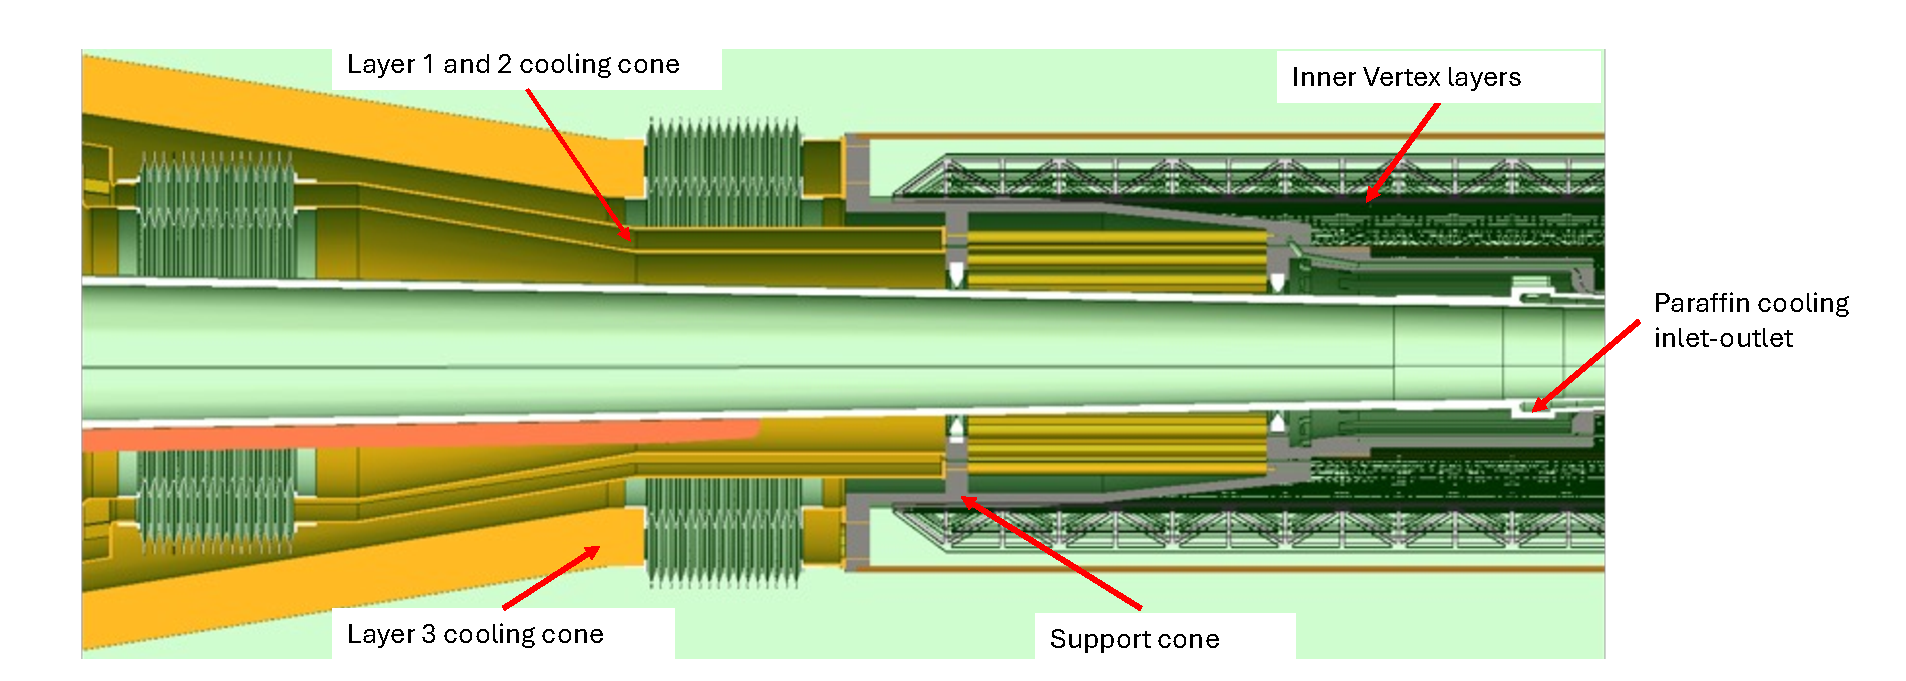
\includegraphics{Physics/MachineDetectorInterface/Figs/vertex-beampipe-integration.pdf}}
\caption{Longitudinal section of the beam pipe and inner vertex layers. 
The dark gray object is the conical support of the vertex detector, which is supported by the conical beam pipe. 
The inlet/outlet paraffin of the central chamber cooling manifolds are visible at the edge of the support cone.
The orange structures represent the cooling cones.}
\label{fig:zoom_vtx_beampipe}
\end{figure}

The luminosity monitor is described in Section~\ref{sec:LumiCal}.
It consists of two cylindrical devices, placed at about 1\,m away from the IP, on either side of the IP.
Each device spans a sensitive radial coverage between 54 and 115\,mm from the beamline plus a service region from 115 to 145\,mm, 
which houses the electronics readout, cables, and cooling. 
In order to achieve the desired accuracy of $10^{-4}$ in the measurement of the luminosity, 
the calorimeter has a stringent requirement on the knowledge of its boundaries.
In particular, the relative positioning of the two sides along the $z$ axis needs to be known with a precision of $\pm 100$\,$\mu$m and, 
once assembled, the calorimeter must be a rigid hollow cylinder. 
This is guaranteed by dimensioning the bellows of the beam pipe such that their external dimensions are smaller than the internal calorimeter bore
and such that it could possibly slide inside.
The beam pipe has been carefully designed to minimise the material effects on particles reaching the luminosity calorimeter. 
In fact, the material budget ranges from approximately 0.07\,$X_0$ to 0.5\,$X_0$ (Fig.~\ref{fig:material_budget_Gold_5mum}). 
The maximum values, driven by the AlBeMet cooling manifolds, are at a safe distance from the 50\,mrad LumiCal acceptance cone. 
The design of the cooling manifolds has been optimised to limit the effects of showers originating from electrons scattering in the beam pipe. 
Ongoing studies show that the impact on the luminosity measurement is limited.

The IR magnet system~\cite{FCC-PED-FSR-Vol2} includes the final focus quadrupoles, the compensating solenoid, the screening solenoid, 
and magnetic correctors for IR tuning. 
%
The limited space available constitutes a challenge to the design of the IR magnet system,
currently envisaged to fit in an envelope of 100\,mrad around the $z$ axis.
The system design includes a cryostat partially located inside the detector, 
surrounding the compensating solenoid and the first final focus quadrupole (QC1),
which is itself embedded in the screening solenoid (for the part inside the detector).
It also includes the second final focus quadrupole (QC2), starting 0.30\,m upstream of QC1.

\subsection{Integration and alignment}

The accelerator and detector components that are placed within $\pm 1.5$\,m from the IP are mounted in a single rigid structure, 
which provides a cantilevered support for the pipe and avoids loads on the thin-walled central chamber during assembly. 
This rigid structure also supports the LumiCal and the vertex detector (Fig.~\ref{fig:support_cyl}).
The support tube is an empty cylindrical structure made of a 4\,mm honeycomb structure interleaved within two 1\,mm thick carbon fibre walls. 
It is longitudinally split in two halves and is complemented by two aluminium flanges and two endcaps that support the LumiCal and the beam pipe. 
Six aluminium ribs are fixed inside the tube in order to support the outer vertex layers. 

\begin{figure}[h!]
\centering
\includegraphics[width=0.85\linewidth]{Physics/MachineDetectorInterface/Figs/Optics_241_Assembly_IR_V3_1_V1.png}
\caption{Support tube showing the beam pipes and bellows, the vertex detector with air-cooling cones, the luminosity detector, 
and, in brown, the vacuum chambers internal to the cryostat (not shown).}
\label{fig:support_cyl}
\end{figure}

A structural analysis, performed to calculate the stress and displacement of each part of the support tube
taking into account the estimated weights of detector elements, including services material,
shows that the structural resistance is safely respected.

The insertion of the support tube in the detector is foreseen either with a few sleds or with longitudinal rails fixed to its external surface. 
A possible option could then be to slide these sleds (rails) inside hollow carbon fibre rails, 
permanently fixed on the inside wall of the tracker to guarantee the structural rigidity while inserting the support tube. 
The corresponding calculations and simulations are beyond the scope of this feasibility study.

The alignment and monitoring device~\cite{Watrelot:2894663} is composed of three main subsystems:

\begin{itemize} 

\item The deformation monitoring system is capable of monitoring the shape of the screening solenoid support, 
which is then used as a reference~\cite{Watrelot_2023}. 
It exploits 
in-line multiplexed and distributed frequency scanning interferometry (IMD-FSI)~\cite{10.1117/12.2529157} 
to monitor sections of optical fibres firmly installed on the inner surface of the screening solenoid support.
This system occupies no more than 5\,cm$^{3}$ within the assemblage and requires an interface with the endcap of the first final focus quadrupole.

\item At the end of each fibre used in the deformation monitoring system, 
a mirror is installed to redirect the laser beam towards the centre of the assemblage, 
targeting the final focusing quadrupoles, the beam position monitors (BPMs), the LumiCal, 
and any other component that requires position monitoring. 
This subsystem is very similar to the FSI heads installed on the low-$\beta$ quadrupoles in the HL-LHC MDI~\cite{MainaudDurand:2667534}. 
The corresponding distance measurements monitor the position of the inner components relative to the cryostat. 
 
\item Finally, to ensure the alignment of both sides of the MDI with respect to each other, 
a long-range alignment system is foreseen, also based on FSI but with a different optical setup to enable longer-distance measurements. 

\end{itemize} 

A dense network of such measurements around the detector provides a continuous link between the endcaps of the QC1 on each side of the MDI, 
which serve as the reference surface for the cylinder monitored by the deformation system. 
Reference points are placed on the supporting feet of the detector, 
easy to access for a technician or a robot, 
and used to link to the cavern survey network and the rest of the accelerator.

A network of Frequency Scanning Interferometry is proposed for the alignment of the inner tracker. 
This network will be implemented similarly to what has been done for the ATLAS SemiConductor Tracker~\cite{gibson2006multi}, 
but with the latest version of the technology, more compact and precise. 
This system also allows the measurement of the positions of the LumiCal and of the beam pipe relative to the FFQs.

\subsection{Maintenance and detector opening}

Periodic (or exceptional) detector maintenance requires, in general, access to the internal subsystems, known as `opening the detector'. 
The design of the MDI region must carefully anticipate the intertwined requirements from the civil engineering, the machine, and the detector.  
Three opening scenarios, with their own advantages and drawbacks, have been examined.

\begin{figure}[ht]
\centering
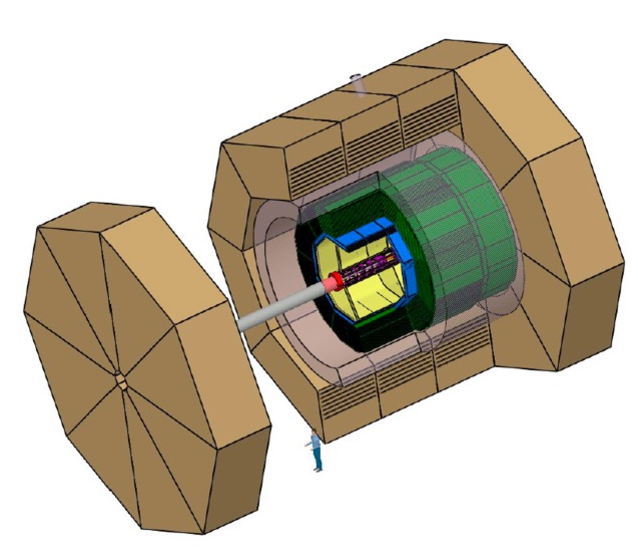
\includegraphics[width=0.49\textwidth]{Physics/MachineDetectorInterface/Figs/Longitudinal.pdf}
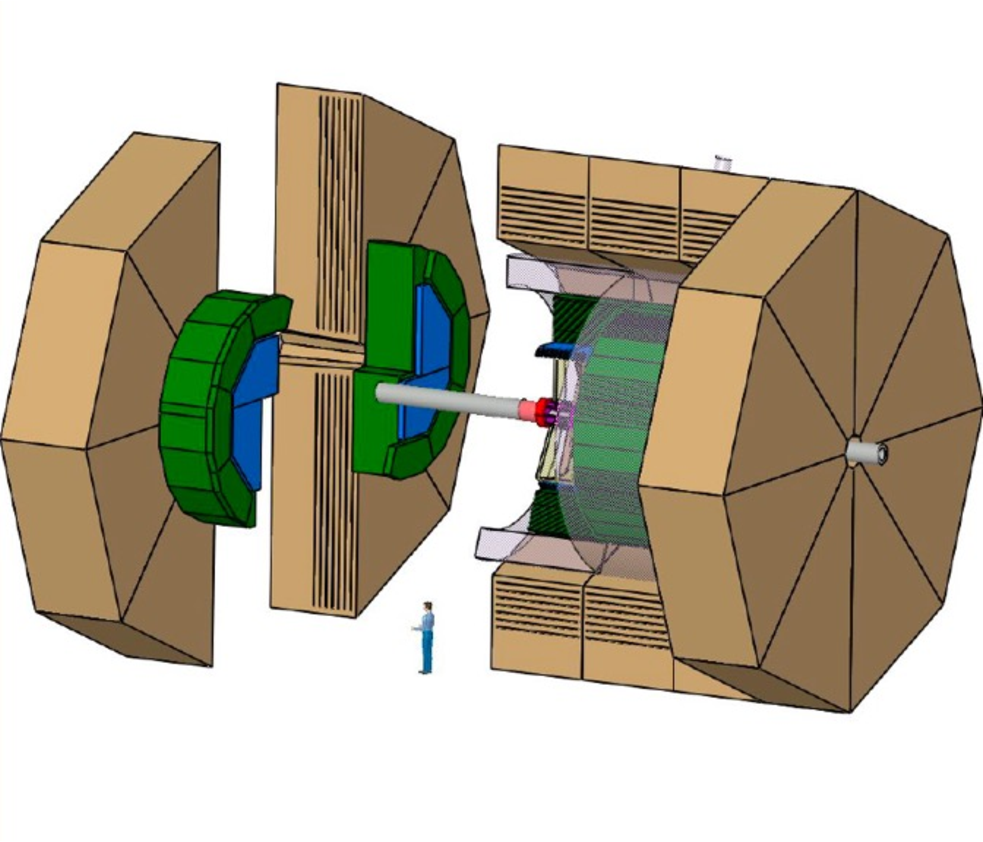
\includegraphics[width=0.49\textwidth]{Physics/MachineDetectorInterface/Figs/diagonal.pdf}
\caption{Longitudinal (left) and short longitudinal plus transversal endcap (right) detector opening}
\label{fig:Detector_openings}
\end{figure}

\begin{enumerate}

\item In a first scenario, the two endcap calorimeters are moved along the $z$ axis to disengage them from the barrel, 
as displayed in the left panel of Fig.~\ref{fig:Detector_openings}, 
by a couple metres if only access to the central tracker is needed 
and by up to 7\,m if the tube supporting the LumiCal, the vertex detector, and the central vacuum chamber requires extraction (and re-insertion). 
The mechanical stability of the final focus quadrupoles requires rigid supports, as close as possible to the detector boundaries. 
These supports, if fixed, would make the longitudinal opening of the detector endcaps  impossible. 
Removable supports would then need to be designed to allow safe removal of the FFQs, 
and a quick re-installation and alignment following the access to the inner detectors. 
In this scenario, in addition to the re-alignment issue, the beam-pipe vacuum is broken. 
As the removal of the FFQs from inside the detector would first require the removal of other machine elements just behind them, 
this scenario can be envisaged only for medium or long machine shutdowns (several weeks or months), 
as done with the BELLE~II detector at SuperKEKB.

\item A second option involves vertically splitting the detector endcaps, allowing opening without removing the FFQs. 
In this scenario, the two split endcaps are first moved longitudinally for about 2\,m and
then moved from the beamline in the transverse direction, as shown in the right panel of Fig.~\ref{fig:Detector_openings}. 
The FFQs could stay cold, with the beam pipe under vacuum. 
This scenario could be very effective in the case of a quick access. 
The only constraint from the machine side is to keep all the services needed by the FFQs 
(supports, vacuum, cryogenics, powering) 
in the shadow of the FFQs, i.e., inside the detector forward acceptance cone. 
The main drawback is the serious impact on the detector acceptance, 
as splitting the endcaps creates a dead zone in the vertical plane 
and may imply a complete recalibration of the calorimeter angular acceptance determination.
    
\item A third, currently preferred, possibility consists of moving the complete detector along the $x$ axis, away from the beamline. 
As in the first scenario, this requires a disconnection of the internal FFQs from the rest of the machine, 
but allows them to be kept inside the detector. 
The FFQs can then be easily removed without touching any other machine element, 
before proceeding to a longitudinal opening of the endcaps without any obstacle. 
The detector integrity is preserved and, although the beam vacuum is broken and a re-alignment of the FFQs is needed, 
relatively short access periods (few weeks) can be envisioned. 
As the FCC-ee detectors have a diameter of typically 12\,m, 
this scenario requires enough transverse free space on one side of the detector, 
which is currently not available in the two small experiment caverns (Section~\ref{sec:caverns}). 
Another location for the balconies (in green on Fig.~\ref{small_cavern}, Chapter~\ref{sec:caverns}) may have to be found in these caverns, 
e.g., by placing all of them on the other side of the detector, 
and a small additional alcove (typically 25\,m long and a few metres deep) might also be needed, 
depending on the exact transverse size of the detector. 
Designing the small caverns so that their axis can be transversely displaced from the beamline by a few metres, 
if compatible with the size of the specialised FCC-hh detectors (Section~\ref{sec:caverns}), 
would alleviate the need for such an alcove.

\end{enumerate}

Technical mitigation solutions for the drawbacks of these three scenarios will be investigated in detail during the next phase of the study.

\subsection{Beam-induced backgrounds in the detectors}
\label{sec:MDI_backgrounds}

The beam-induced backgrounds in the detectors arise from two categories of sources: 
those generated by processes involving only a single beam, 
and those generated by the interactions between the two beams at each IP, usually called luminosity backgrounds.

Although the collimation system and absorbers remove the bulk of the particles produced by single beams 
(electrons/positrons and photons) 
before they can hit the detectors, 
some background may remain because the particles can scatter off them. 
Elastic and inelastic interactions of the beam with the molecules of the residual gas produce scattered particles, 
deviating from the original orbits, as well as photons from inverse-Compton scattering. 
Showers may also be produced for a very small fraction of events. 

Intra-beam particle interactions, also known as Touschek scattering, are negligible at FCC-ee, 
given that they are suppressed by a large energy factor in comparison to lower energy colliders, 
such as SuperKEKB and DA$\Phi$NE. 
Synchrotron radiation~\cite{Andre:2024bfm} has been simulated with \textsc{Bdsim}~\cite{Nevay} and the \textsc{Geant4}~\cite{Allison} toolkit. 
The bulk of SR is emitted almost collinearly with the beam, 
and the IR optics keeps it away from the detector sensitive layers. 
Magnet misalignments, imperfections, and beam tails, however, may cause SR to reach the detector. 
Studies are ongoing to optimise the design and the position of dedicated masks 
(a few metres upstream of the detector) 
in order to minimise the effects of SR in the detector.

A variety of processes such as space-charge effects, beam instabilities, interaction with residual gas, 
intra-beam scattering, magnet misalignments, and magnetic field errors can lead to the population of a beam halo, 
potentially leading to beam particle losses.
These particles are mostly intercepted by the collimators located in the dedicated section of the collider~\cite{FCC-PED-FSR-Vol2}, 
following the approach used for LHC~\cite{bruce2014simulations}.  
The relevant studies have been performed with the \textsc{Xsuite-Bdsim} simulation tool~\cite{Abramov:2024uas,Broggi:2024ocw}.
The vast majority of the beam halo losses in the MDI are intercepted by the SR collimators,
so that no losses are observed beyond the last SR collimators before the IPs, in all cases.
The background contribution from beam halo particles that leak from the beam halo collimation system is,
therefore, not expected to be an issue. 
Tertiary collimators have been included upstream of the SR collimators, 
strongly further reducing the effects of residual losses.

Beam-gas interactions depend on the residual gas pressure profile in the rings and on the outgassing materials inside the vacuum chambers. 
Simulations of the beam-gas interactions have been performed with \textsc{Molflow+}~\cite{Kersevan:IPAC2019-TUPMP037}, 
with a residual gas pressure profile resulting from 1\,h beam conditioning at a full nominal current of 1.27\,A at the \PZ pole. 
Within $\pm 500$\,m from the IP, 
the gas composition is 85\% hydrogen, 10\% carbon monoxide, and 5\% carbon dioxide, 
at an average pressure of $10^{-11}$\,mbar and spikes of $10^{-8}$\,mbar in the vicinity of the SR absorbers. 
This vacuum level, conservatively estimated at the beginning of the machine commissioning, is expected to progressively improve over time. 
Preliminary results obtained with \textsc{Fluka} indicate that the dose and fluence due to beam-gas interactions within $\pm 500$\,m from the IP
in the \PZ pole run are not the leading contributors: 
for a pressure profile resulting from only one hour of beam conditioning, 
the estimated dose and fluence in the innermost vertex detector layers are as low as 3\,kGy/year 
and $\sim 7 \times 10^{11}$\,cm$^{-2}$/year, further decreasing with increasing conditioning.

The most relevant luminosity background arises from incoherent pairs creation (IPC)~\cite{Ciarma:2023iat}, 
a class of interactions between two photons emitted by a single electron and a single positron at the IP, $\epem \to (\epem) \epem$. 
The simulation of these backgrounds has been performed with \textsc{GuineaPig}~\cite{Schulte:1998au} 
and interfaced to \textsc{Key4HEP} (Section~\ref{sec:software}). 
The resulting $\epem$ pairs are predominantly produced in the forward direction, with small transverse momenta. 
Although the production cross section is large, only a small fraction of these particles are in the detector acceptance, 
as shown in Fig.~\ref{fig:ipc} for the \PZ-pole and $\ttbar$ runs;
a few others hit the region where the two beam pipes bifurcate (crotch) and scatter off the detector.

\begin{figure}[ht]
\centering
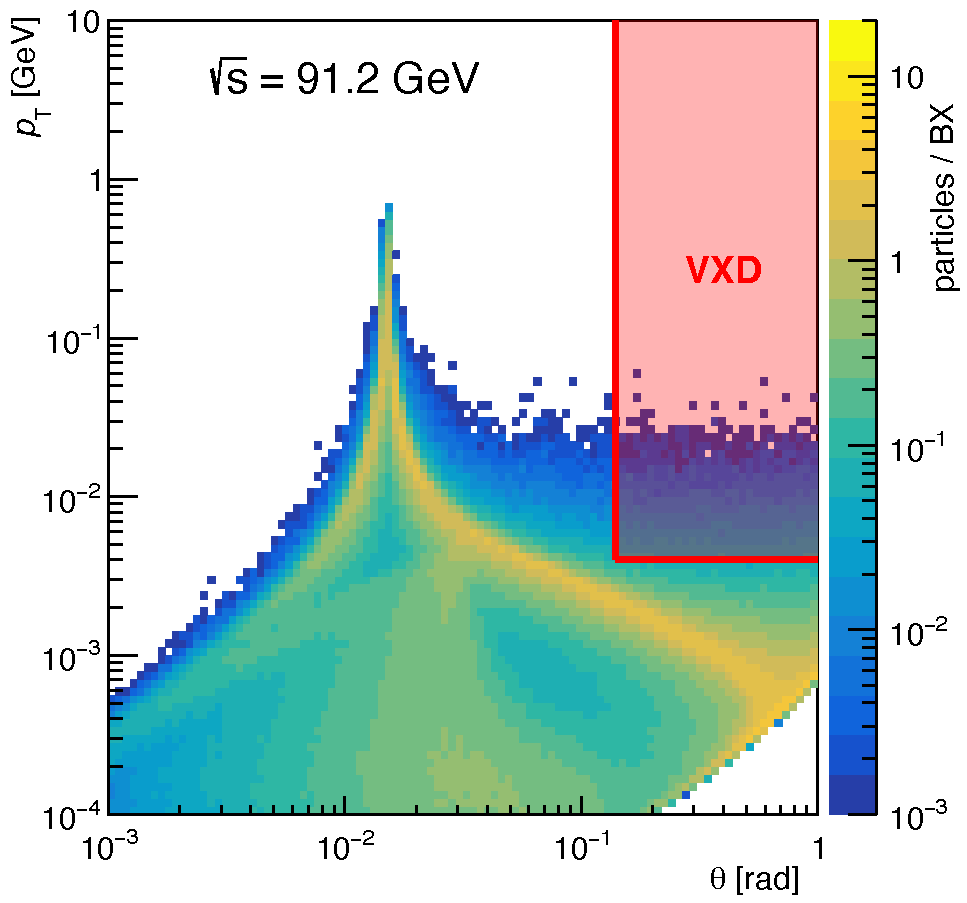
\includegraphics[width=0.4\linewidth]{Physics/MachineDetectorInterface/Figs/c00_Z-CL.pdf}
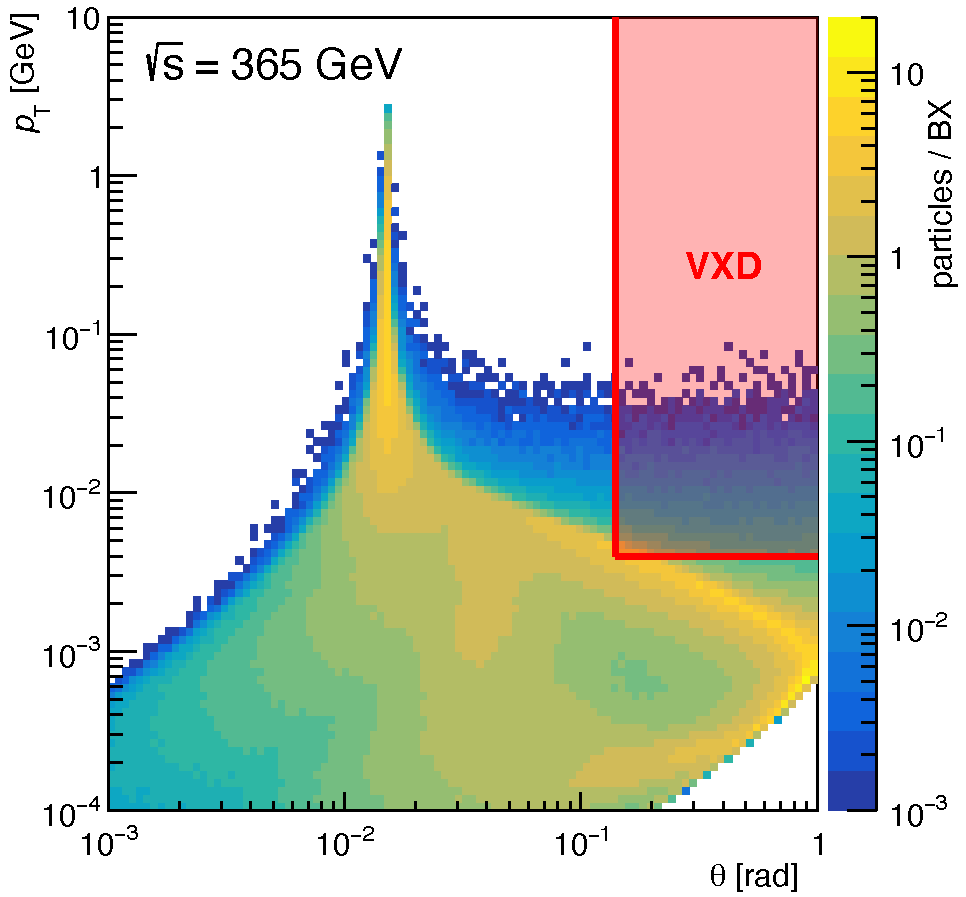
\includegraphics[width=0.4\linewidth]{Physics/MachineDetectorInterface/Figs/c00_T-CL.pdf}
\caption{Number of IPC particles produced for each FCC-ee bunch crossing, 
as a function of their transverse momentum and polar angle, 
for the \PZ (left) and $\ttbar$ (right) working points. 
The area limited by the red lines represents the acceptance of the vertex detector.}
\label{fig:ipc}
\end{figure}

The largest effect occurs in the \PZ-pole run, given its instantaneous luminosity, the highest of the FCC-ee programme.
In the innermost layer of the IDEA vertex detector,
the hit rate reaches about 70\,MHz/cm$^2$, for an average of 5 pixels per cluster, 
which imposes a rather stringent requirement on the readout electronics of the order of 200\,MHz/cm$^2$
with, conservatively, a safety factor of~3.
In the IDEA drift chamber, 
where the pairs created by several successive bunch crossings need to be integrated during the drift time (400\,ns), 
the occupancy is about 7\%. 
Incoherent pairs may also reach larger radii and their effects have been studied for the ALLEGRO liquid Argon electromagnetic calorimeter. 
The first layers of the calorimeter are the most affected, 
but the effect can be largely mitigated by setting a minimum readout energy threshold of 20\% of the energy released by a minimum ionising particle, 
resulting in an occupancy of 0.03\% in the barrel and 0.2\% in the endcaps.

Radiative Bhabha (RB) scattering, $\epem \to \epem \PGg$, 
is another important luminosity background that may severely affect the superconducting FFQs. 
Radiative Bhabha events were generated with \textsc{BBBrem}~\cite{KLEISS1994372} and \textsc{GuineaPig}, 
and processed by \textsc{Fluka}~\cite{FLUKA, FLUKA:2015, FLUKA2021}. 
Their study shows that a substantial annual dose of power is deposited in QC1, 
which necessitates a tungsten shielding of approximately 2\,mm around the beam pipe to protect the superconducting magnets.
This shielding decreases the annual dose power deposition peak value to about 3\,MGy (a reduction by an order of magnitude)
and the deposited power density to about 1.5\,mW/cm$^3$.
These values are compatible with the design dose limit of 30\,MGy for the full magnet lifetime and the quench limit of 10--20\,mW/cm$^3$ adopted at the LHC.
Other radiation sources contributing to the energy deposition in QC1, 
like beam-gas scattering, incoherent pair creation or synchrotron radiation, 
still need to be carefully evaluated at the FFQs.
They are expected, however, to be much more benign than radiative Bhabha events.
The integration of this shielding with the design of QC1 will be performed in the next phase of the study.

The total ionisation dose (TID) and the 1\,MeV neutron-equivalent (n$_\text{eq}$) fluence 
from the main radiation sources in the \PZ-pole operational mode (i.e., RB and IPC) 
have been estimated in the IDEA interaction region with \textsc{Fluka}, 
and are displayed in Fig.~\ref{fig:TID_IR}.
The peak annual dose and fluence in the inner vertex detector are at the level of a few tens of kGy and a few 10$^{13}$\,cm$^{-2}$, 
respectively, for the innermost layers. 
These numbers are compatible with most of the technologies currently under consideration for the monolithic active pixel sensors. 
At higher centre-of-mass energies, the TID and fluence are expected to be smaller, given the reduced instantaneous luminosity. 

\begin{figure}[ht]
\centering
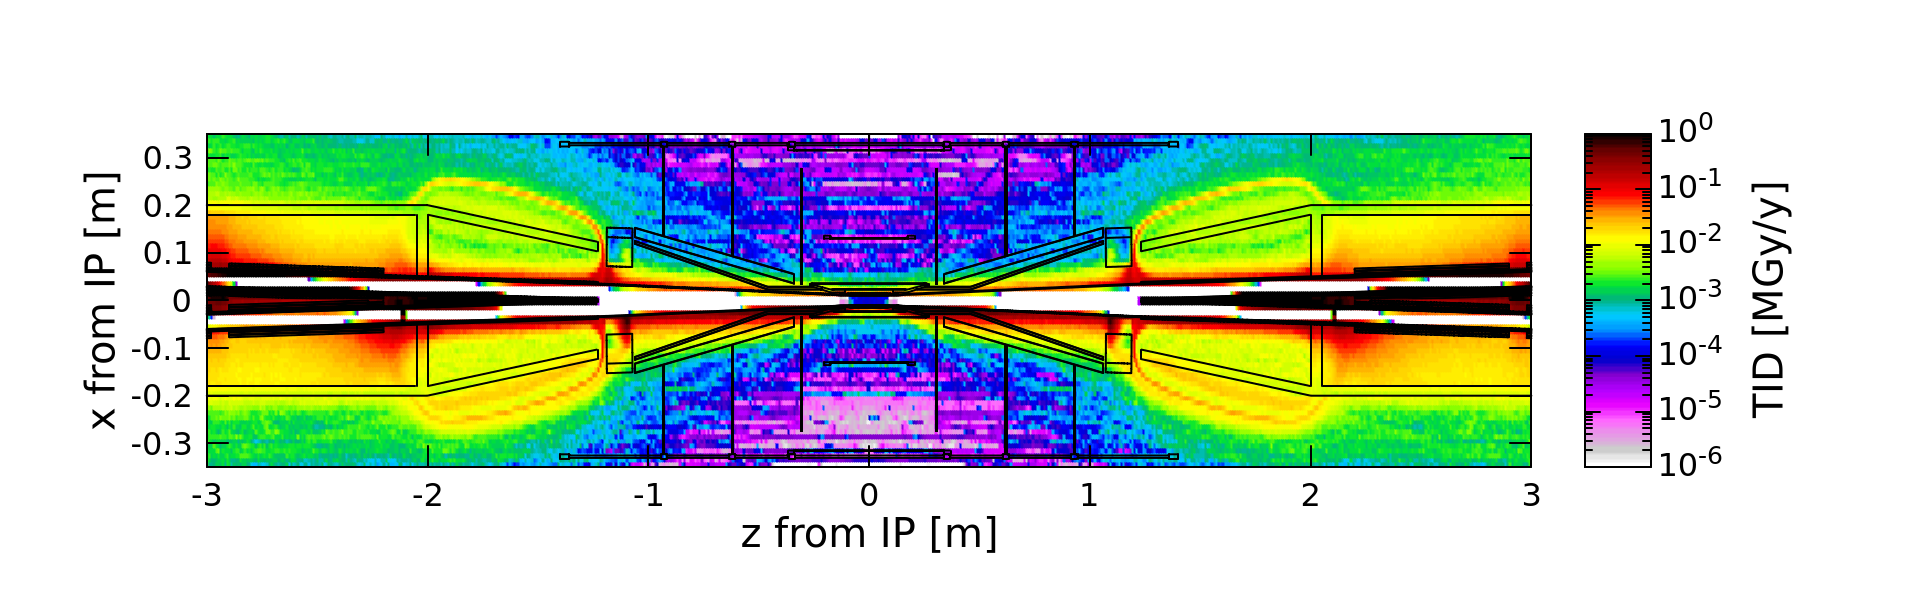
\includegraphics[width=0.99\linewidth]{Physics/MachineDetectorInterface/Figs/TID.png}
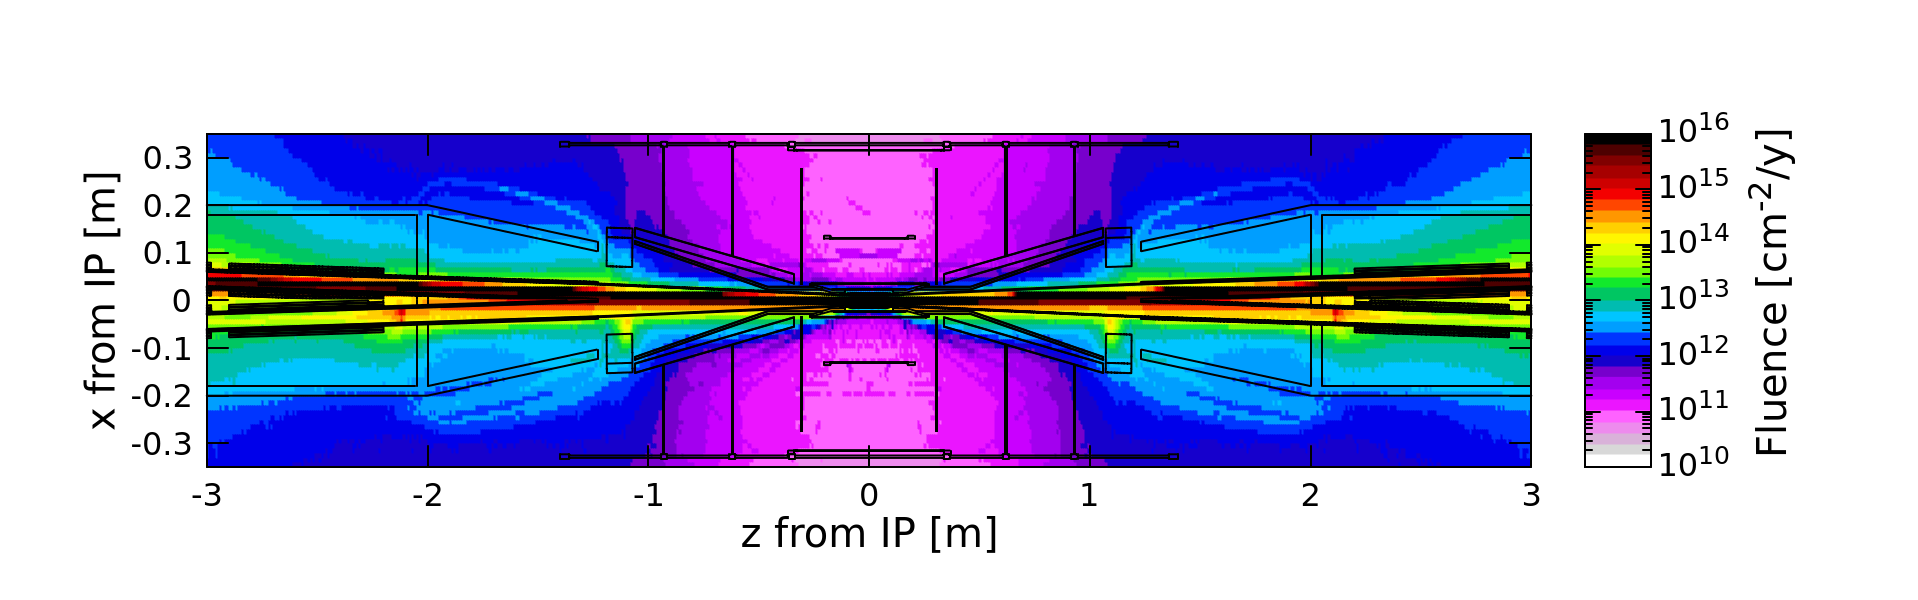
\includegraphics[width=0.99\linewidth]{Physics/MachineDetectorInterface/Figs/IR_fluence.png}
\caption{Total ionisation dose (top) and 1~MeV\,n$_\text{eq}$ fluence (bottom) in the interaction region of the IDEA detector.}
\label{fig:TID_IR}
\end{figure}

\subsection{Implementation tests and prototyping}

Design and simulation studies must be complemented by actual prototyping and implementation tests, 
to develop dedicated setups and evaluate technical solutions to the integration challenges. 
The following activities are proposed or planned; some are already ongoing.

\begin{itemize}
    
\item The realisation of a full scale mock-up of the beam pipes of the IR is being carried out at INFN (LNF and Pisa). 
This study includes the integration of the vertex and LumiCal detectors in the support tube, 
with particular emphasis on the paraffin and water cooling of the pipes and on the air cooling of the inner vertex detector. 
This activity is fully integrated with the R\&D carried out in the ECFA DRD8 Working Group~\cite{DRD8}.

\item The experimental validation of the alignment system of the FFQ is ongoing with the FSI system at CERN, 
using a 1:2 mock-up of the beam pipes and cryostat.

\item The design of the screening anti-solenoid and
and the production of QC1 corrector prototypes 
are proposed at the Brookhaven National Laboratory (BNL), 
leveraging their `direct winding technology'~\cite{Parker:2012pla}.

\item The fabrication of a High Temperature Superconducting (HTS) magnet is proposed by LAPP Annecy for the final quadrupole QC1, 
together with its integration with the water-cooled beam-pipe.

\end{itemize}

In summary, a lot of progress has been made in the past years. 
The layout has been significantly improved by reducing the material budget in front of the LumiCal 
and also through a careful design of the cooling manifolds, re-engineered in AlBeMet162 material. 
The feasibility of the inner vertex detector cooling has been validated 
and the routings of its services have been designed and integrated with those of the beam pipe.
More studies are on the way to optimise the design and confirm its validity experimentally. 
A careful analysis of the detector maintenance and FFQ integration has been performed, 
leading to the identification of the main optimisation issues to be tackled during the next phase of the study. 
An alignment strategy has been outlined, based on the technology planned for HL-LHC. 
Finally, the study of the beam-induced backgrounds and the evaluation of the main radiation doses and fluences in the IR region 
led to the development of mitigation measures, like the design of the collimation system and SR shielding.

\subsection{Outlook}

Studies carried out during the Conceptual Design Study and the Feasibility Study have converged to a baseline MDI design with satisfactory overall performance. 
Further investigations to consolidate this design and to improve its performance will be performed. 
Refinements will also be needed when actual detector proposals are finalised.   

Several options are currently considered for the QC1 cryostat design. 
Most importantly, a choice will be made for the operating temperature of the cooling scheme, 
among three options: 
1.9-2.1\,K in pressurised He~II; 
4.5\,K for supercritical He; 
or 10--20\,K for He gas forced flow. 
Another important design decision concerns the dimensions of the cryostat, 
which currently covers a cone of 100\,mrad around the $z$ axis. 
While the forward acceptance of the detector calorimetry would benefit from a smaller cryostat,
the operability of the collider, and the integrated luminosity, would advocate for more relaxed dimensions, 
calling for a complete optimisation study.  

In the baseline MDI design, 
the detector solenoid field of 2\,T is `locally' compensated with $-5$\,T solenoids placed within $\pm\ell^*$ around the IP. 
The performance of an alternative `non-local' scheme, 
with $-2$\,T solenoids positioned outside the detector at about $\pm 20$\,m from the IP~\cite{Ciarma:2024mri}, 
will be studied and compared to that of the baseline. 
First observations show that the non-local scheme might achieve a better residual vertical emittance, 
opening the possibility to increase the strength of the detector solenoid field to 3\,T. 
An adverse consequence of the non-local scheme seems to be a higher spin depolarisation, 
so that further investigations are needed to preserve the possibility of beam-energy calibration with resonant depolarisation (Chapter~\ref{sec:epol}). 

The main beam-induced background sources have been studied during the Feasibility Study, 
with the exception of the injection backgrounds and thermal photons, which will have to be included. 
The studies of the impact of all backgrounds in the data taking and in the physics performance will be finalised, 
and proposed mitigation solutions will be consolidated. 
To this aim, the \textsc{Fluka} software interface between the simulation of the machine backgrounds and the simulation of the detector will be refined. 
A deeper understanding will be sought of the synchrotron radiation background mitigation, 
in particular the positioning of the SR masks or the tolerances of the machine elements that might impact the detectors, 
such as the alignment of the FFQs, the collimators, and the vacuum system.  
More generally, the effectiveness of the shielding elements to protect the detector and the superconducting FFQ magnets will be thoroughly evaluated.

As the design of the sub-detectors (e.g., vertex detectors, luminometers, superconducting pipes, supporting structures) 
and of the accelerator components (e.g., beam position monitors, vacuum pumps, remote vacuum connections, cryostat supporting structures) 
get finalised, their integration, as well as the impact on the maintenance and assembly of the interaction region, will be established in more detail. 
Finally, methods for the alignment, the opening, and the maintenance of the detector and accelerator elements 
will be developed, and possible consequences on the cavern dimensions will be evaluated.